\documentclass[14pt]{extbook}
\usepackage{multicol, enumerate, enumitem, hyperref, color, soul, setspace, parskip, fancyhdr} %General Packages
\usepackage{amssymb, amsthm, amsmath, latexsym, units, mathtools} %Math Packages
\everymath{\displaystyle} %All math in Display Style
% Packages with additional options
\usepackage[headsep=0.5cm,headheight=12pt, left=1 in,right= 1 in,top= 1 in,bottom= 1 in]{geometry}
\usepackage[usenames,dvipsnames]{xcolor}
\usepackage{dashrule}  % Package to use the command below to create lines between items
\newcommand{\litem}[1]{\item#1\hspace*{-1cm}\rule{\textwidth}{0.4pt}}
\pagestyle{fancy}
\lhead{Makeup Progress Quiz 3}
\chead{}
\rhead{Version C}
\lfoot{1648-1753}
\cfoot{}
\rfoot{Summer C 2021}
\begin{document}

\begin{enumerate}
\litem{
Solve the equation below. Then, choose the interval that contains the solution.\[ -17(-12x + 3) = -18(7x -14) \]\begin{enumerate}[label=\Alph*.]
\item \( x \in [-1.29, -0.35] \)
\item \( x \in [0.2, 0.65] \)
\item \( x \in [-3.56, -1.75] \)
\item \( x \in [0.83, 1.17] \)
\item \( \text{There are no real solutions.} \)

\end{enumerate} }
\litem{
Find the equation of the line described below. Write the linear equation in the form $ y=mx+b $ and choose the intervals that contain $m$ and $b$.\[ \text{Parallel to } 3 x - 4 y = 12 \text{ and passing through the point } (6, 9). \]\begin{enumerate}[label=\Alph*.]
\item \( m \in [0.67, 1.16] \hspace*{3mm} b \in [4.47, 5.43] \)
\item \( m \in [1.31, 1.56] \hspace*{3mm} b \in [4.47, 5.43] \)
\item \( m \in [-0.91, -0.16] \hspace*{3mm} b \in [12.68, 13.77] \)
\item \( m \in [0.67, 1.16] \hspace*{3mm} b \in [-5.48, -3.1] \)
\item \( m \in [0.67, 1.16] \hspace*{3mm} b \in [2.96, 3.8] \)

\end{enumerate} }
\litem{
Find the equation of the line described below. Write the linear equation in the form $ y=mx+b $ and choose the intervals that contain $m$ and $b$.\[ \text{Perpendicular to } 6 x - 7 y = 7 \text{ and passing through the point } (-6, -8). \]\begin{enumerate}[label=\Alph*.]
\item \( m \in [-0.99, -0.1] \hspace*{3mm} b \in [-15.17, -14.25] \)
\item \( m \in [-1.91, -1.14] \hspace*{3mm} b \in [-15.17, -14.25] \)
\item \( m \in [-1.91, -1.14] \hspace*{3mm} b \in [-4.17, -1.8] \)
\item \( m \in [0.93, 1.7] \hspace*{3mm} b \in [-1.39, -0.24] \)
\item \( m \in [-1.91, -1.14] \hspace*{3mm} b \in [14.93, 15.47] \)

\end{enumerate} }
\litem{
Write the equation of the line in the graph below in Standard Form $Ax+By=C$. Then, choose the intervals that contain $A, B, \text{ and } C$.
\begin{center}
    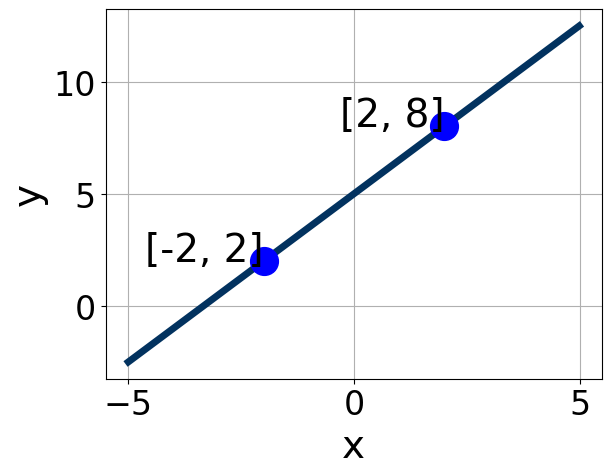
\includegraphics[width=0.5\textwidth]{../Figures/linearGraphToStandardCopyC.png}
\end{center}
\begin{enumerate}[label=\Alph*.]
\item \( A \in [-2.9, -0.3], \hspace{3mm} B \in [0.01, 1.56], \text{ and } \hspace{3mm} C \in [-6, -2] \)
\item \( A \in [-7, -1.8], \hspace{3mm} B \in [2.87, 3.77], \text{ and } \hspace{3mm} C \in [-16, -6] \)
\item \( A \in [0, 4.8], \hspace{3mm} B \in [2.87, 3.77], \text{ and } \hspace{3mm} C \in [-16, -6] \)
\item \( A \in [0, 4.8], \hspace{3mm} B \in [-3.02, -2.9], \text{ and } \hspace{3mm} C \in [10, 20] \)
\item \( A \in [-2.9, -0.3], \hspace{3mm} B \in [-1.54, -0.99], \text{ and } \hspace{3mm} C \in [4, 11] \)

\end{enumerate} }
\litem{
Solve the linear equation below. Then, choose the interval that contains the solution.\[ \frac{-8x + 7}{4} - \frac{-5x + 3}{7} = \frac{-6x -5}{8} \]\begin{enumerate}[label=\Alph*.]
\item \( x \in [-0.65, 0.35] \)
\item \( x \in [14.8, 21.8] \)
\item \( x \in [3.63, 4.63] \)
\item \( x \in [4.23, 6.23] \)
\item \( \text{There are no real solutions.} \)

\end{enumerate} }
\litem{
First, find the equation of the line containing the two points below. Then, write the equation in the form $ y=mx+b $ and choose the intervals that contain $m$ and $b$.\[ (9, 5) \text{ and } (-11, -8) \]\begin{enumerate}[label=\Alph*.]
\item \( m \in [-0.1, 2.1] \hspace*{3mm} b \in [0.2, 0.9] \)
\item \( m \in [-0.1, 2.1] \hspace*{3mm} b \in [1, 5.7] \)
\item \( m \in [-1.4, 0.2] \hspace*{3mm} b \in [-17.6, -13.7] \)
\item \( m \in [-0.1, 2.1] \hspace*{3mm} b \in [-1.3, 0.7] \)
\item \( m \in [-0.1, 2.1] \hspace*{3mm} b \in [-4.3, -2.4] \)

\end{enumerate} }
\litem{
Write the equation of the line in the graph below in Standard Form $Ax+By=C$. Then, choose the intervals that contain $A, B, \text{ and } C$.
\begin{center}
    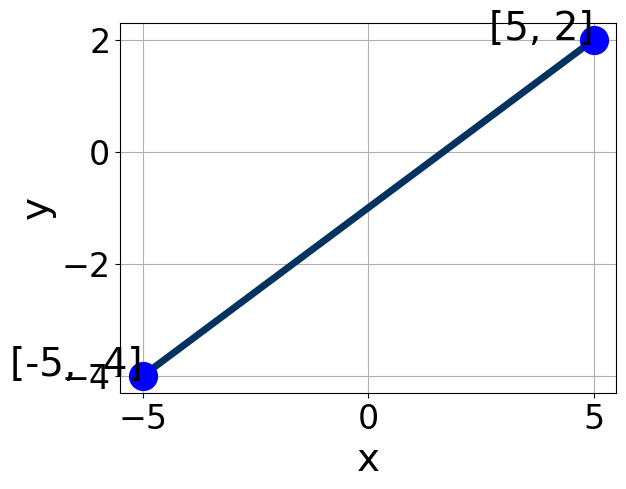
\includegraphics[width=0.5\textwidth]{../Figures/linearGraphToStandardC.png}
\end{center}
\begin{enumerate}[label=\Alph*.]
\item \( A \in [3.8, 4.4], \hspace{3mm} B \in [2.3, 8.6], \text{ and } \hspace{3mm} C \in [-16, -8] \)
\item \( A \in [-3, 0.6], \hspace{3mm} B \in [-1.8, -0.4], \text{ and } \hspace{3mm} C \in [1, 4] \)
\item \( A \in [-3, 0.6], \hspace{3mm} B \in [-0.4, 2.2], \text{ and } \hspace{3mm} C \in [-6, -1] \)
\item \( A \in [-5.7, -3.3], \hspace{3mm} B \in [2.3, 8.6], \text{ and } \hspace{3mm} C \in [-16, -8] \)
\item \( A \in [3.8, 4.4], \hspace{3mm} B \in [-5.3, -3.5], \text{ and } \hspace{3mm} C \in [13, 20] \)

\end{enumerate} }
\litem{
Solve the equation below. Then, choose the interval that contains the solution.\[ -10(8x + 5) = -14(7x + 9) \]\begin{enumerate}[label=\Alph*.]
\item \( x \in [-5.22, -2.22] \)
\item \( x \in [5.78, 10.78] \)
\item \( x \in [-0.99, 3.01] \)
\item \( x \in [-9.78, -6.78] \)
\item \( \text{There are no real solutions.} \)

\end{enumerate} }
\litem{
First, find the equation of the line containing the two points below. Then, write the equation in the form $ y=mx+b $ and choose the intervals that contain $m$ and $b$.\[ (11, 4) \text{ and } (7, -11) \]\begin{enumerate}[label=\Alph*.]
\item \( m \in [3.75, 8.75] \hspace*{3mm} b \in [-42.25, -33.25] \)
\item \( m \in [-8.75, -1.75] \hspace*{3mm} b \in [7.25, 21.25] \)
\item \( m \in [3.75, 8.75] \hspace*{3mm} b \in [-12, 0] \)
\item \( m \in [3.75, 8.75] \hspace*{3mm} b \in [33.25, 42.25] \)
\item \( m \in [3.75, 8.75] \hspace*{3mm} b \in [-23, -16] \)

\end{enumerate} }
\litem{
Solve the linear equation below. Then, choose the interval that contains the solution.\[ \frac{4x -9}{7} - \frac{7x -9}{4} = \frac{-4x -5}{6} \]\begin{enumerate}[label=\Alph*.]
\item \( x \in [-8.28, -2.28] \)
\item \( x \in [1.51, 5.51] \)
\item \( x \in [-3.8, -0.8] \)
\item \( x \in [8.77, 10.77] \)
\item \( \text{There are no real solutions.} \)

\end{enumerate} }
\end{enumerate}

\end{document}